% \pagebreak[4]
% \hspace*{1cm}
% \pagebreak[4]
% \hspace*{1cm}
% \pagebreak[4]


\ifpdf
    \graphicspath{{pic/}}
\else
    \graphicspath{{pic/}}
\fi

\chapter{ Virtual Observatory (VO)}

\begin{lstlisting}[frame=single]
What is the motivation behind Virtual Observatory? Is data avalanche
problem only in astronomy? What is IVOA?  What is Virtual Observatory
architecture, standards and protocols
\end{lstlisting}

\section{ Data avalanche: Opportunity or disaster?}

There are two important trends in current astronomy surveys:

\begin{itemize}

  \item{Size:} The cumulative compressed data holdings of the ESO archive will
    reach 1 PetaByte by 2012 \cite{hanisch2010international}. Projects
    like Large Synoptic Survey Telescope (LSST) will produce about 30
    TB per night, leading to a total database over the ten years of
    operations of 60 PB for the raw data.
   
  \item{Complexity:}  Modern surveys will cover the sky in different wavebands, from
    gamma- and X-rays, optical, infrared, through to radio. The ability
    to crosscorelate these observations toghether may lead to the new
    understanding of physical phenomenas.
\end{itemize}

    Such amount of data is not possible transfer over the network. It
    imply they are heterogenous, distributed and decentralized in nature.


    There is an interesting analogy with the problem (and the
    solution) which had scientist during LEP project at CERN.  Their
    problem was too many documents in different formats. Tim
    Berners-Lee \footnote{ Sir Timothy John "Tim" Berners-Lee. British
      engineer and computer scientist and MIT professor credited with
      inventing the World Wide Web.} designed set of protocols (URIs,
    HTTP and HTML) which allowed link and share documents
    \cite{berners1990worldwideweb}. This was recognized as generaly
    useful and World Wide Web was born. An important role plays the
    World Wide Web Consortium (W3C) in developing Web
    standards. \footnote{Prior to its creation, incompatible versions
      of HTML were offered by different vendors, increasing the
      potential for inconsistency between web pages.}
    
    
\section{International Virtual Observatory Alliance (IVOA)}

   \begin{wrapfigure}{r}{0.5\textwidth}
     \vspace{0pt}
     \begin{center}
       
\includegraphics[width=0.4\textwidth]{ivoamembers}
     \end{center}
     \vspace{-20pt}
     \caption{IVOA members}
     \vspace{-10pt}
   \end{wrapfigure}


    What is neccessary is sets of standards and protocols to deal with
    heterogenous distributed data and the authority which encourages
    their implementation. Such authority is the International Virtual
    Observatory Alliance (IVOA). It comprises 19 VO programs from
    Argentina, Armenia, Australia, Brazil, Canada, China, Europe,
    France, Germany, Hungary, India, Italy, Japan, Russia, Spain, the
    United Kingdom, and the United States and inter-governmental
    organizations (ESA and ESO)\cite{hanisch2010international}.
   
    Standards specifications can be obtained on \url{http://www.ivoa.net/}.

    %% \begin{figure}[!htbp]
    %%   \begin{center}
    %%     \leavevmode
    %%     \ifpdf
    %%     
\includegraphics[height=6cm]{ivoamembers}
    %%     \else
    %%     
\includegraphics[bb = 92 86 545 742, height=6in]{ivoamembers}
    %%     \fi
    %%     \caption{IVOA members}
    %%     \label{FigAir}
    %%   \end{center}
    %% \end{figure}


\section{Architecture}
    The Virtual Observatory is the  “middle layer” framework
    which connects the Resource Layer to the User Layer in a seamless
    and transparent manner. The objective is to improve and unify access to
    astronomical data and services.

    \begin{figure}[!htbp]
      \begin{center}
        \leavevmode
        \ifpdf
        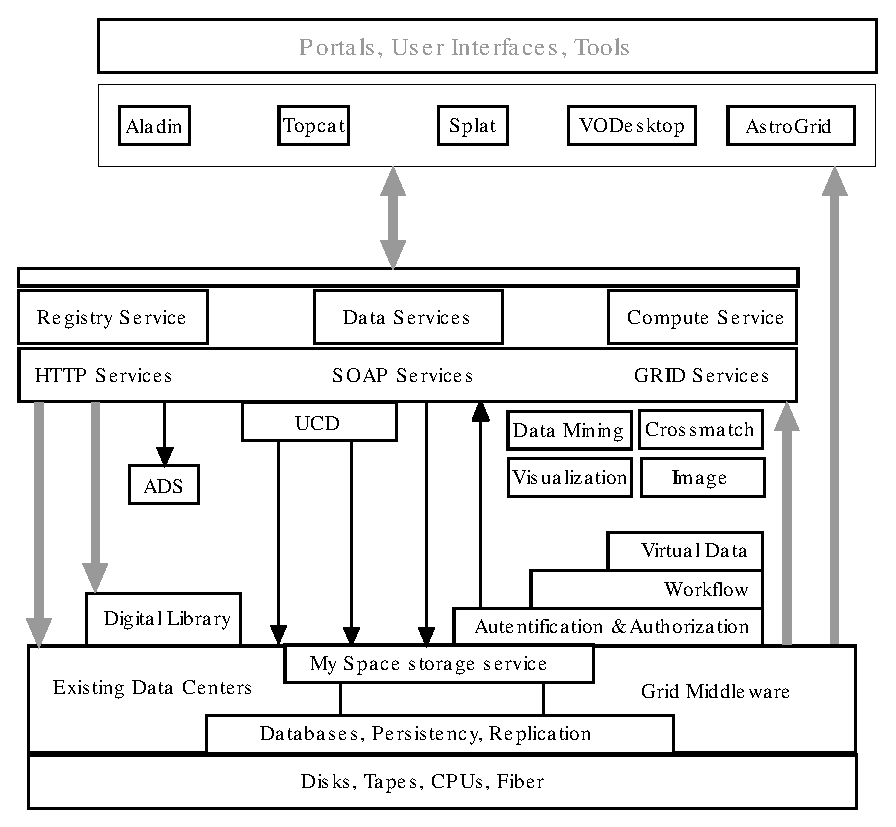
\includegraphics[scale =.6]{architecture}
        \else
        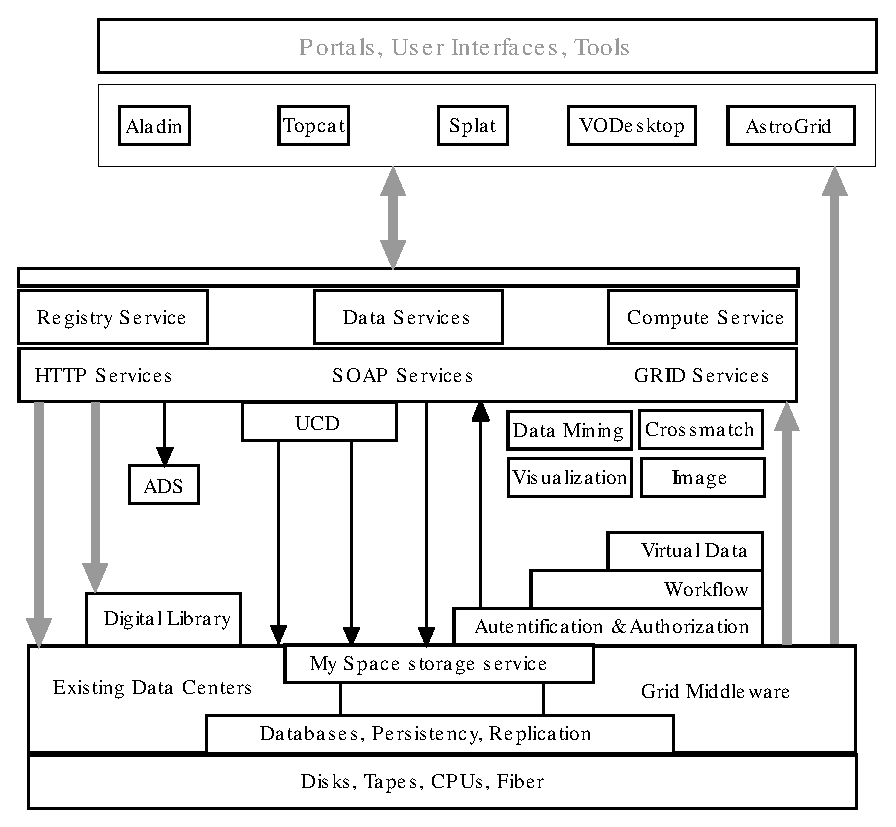
\includegraphics[bb = 92 86 545 742, height=6in]{architecture}
        \fi
        \caption{VO Architecture}
        \label{FigArchitecture}
      \end{center}
    \end{figure}

\clearpage

The Architecture is depicted on the figure \ref{FigArchitecture}.The
level of abstraction goes from top to bottom. Starting with iterfaces,
used by people or applicatian to discover resources.  Next level is
the service layer implemented by standard protocols, followed by the
hardware level where actual data are stored. This onion like structure
hide the complexity of the lower layer and provide data and metadata
to the higher layer. This concept is similar to TCP/IP
\footnote{TCP/IP (Transmission Control Protocol/Internet Protocol).
  The basic communication language or protocol of the Internet.}
protocol.


The essence of VO architecture is service orientation. Each service is
autonomous with well defined defined boundaries. Very important aspect
of VO implementation is the adoption of formats and protocols used in
astronomy (FITS) and computers science (XML \footnote{Extensible
  Markup Language (XML) is a set of rules for encoding documents in
  machine-readable form.} , Web service \footnote{method of
  communication between two electronic devices over a network.} SOAP
\footnote{Simple Object Access Protocol, is a protocol specification
  for exchanging structured information in the implementation of Web
  Services in computer networks.}) for many years. In other words VO
does not reinvent the wheell but it's stands on the shoulders of
giants.


\section{VOResources}

A resource is a general term referring to a VO element that can be
described in terms of who curates or maintains it and which can be
given a name and a unique identifier. Just about anything can be a
resource: it can be an abstract idea, such as sky coverage or an
                                                                   4
instrumental setup, or it can be fairly concrete, like an organization
or a data collection. \cite{bensonivoa}




    \begin{figure}[!htbp]
      \begin{center}
        \leavevmode
        \ifpdf
        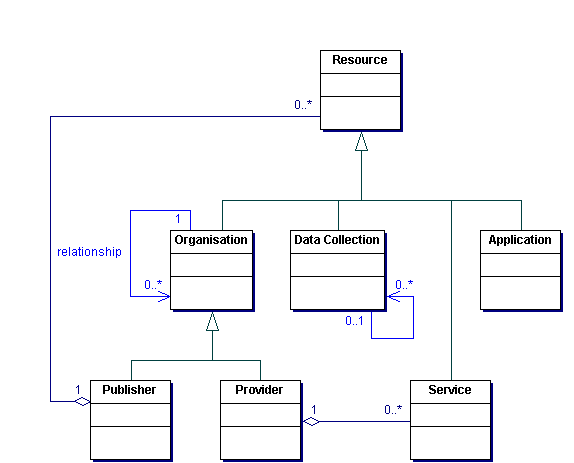
\includegraphics[height=10cm]{resource}
        \else
        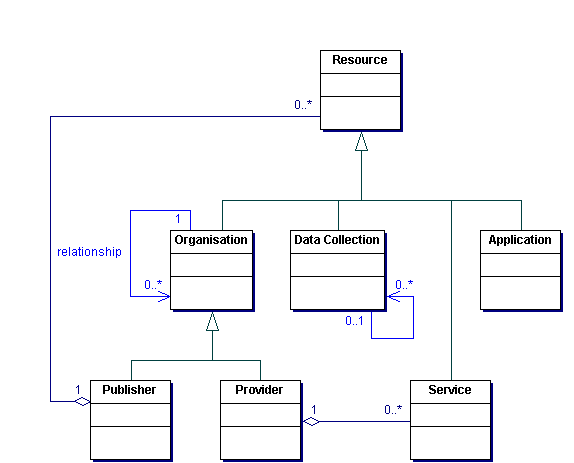
\includegraphics[bb = 92 86 545 742, height=6in]{resource}
        \fi
        \caption{UML diagram of VO-registry}
        \label{FigAir}
      \end{center}
    \end{figure}


Example of resources

\begin{lstlisting}[frame=single]
stilts regquery query="shortName like 'AIASCR'"
regurl=http://registry.euro-vo.org/services/RegistrySearch
ofmt=votable-tabledata > resourceExample.vot
\end{lstlisting}

  \input{resourceExample.vot}



    
\section{VOregistry}
    Is the standard defined by IVOA for registration of VO-Resources

    The IVOA Registry enables users and applications in the User Layer to discover 
    data  and  metadata  collections,  as  well  services  in  the  Resource  Layer.  A 
    resource  is  a  general  term  referring  to  a  VO  element  that  can  be  described  in 
    terms  of  who  curates  or  maintains  it  and  which  can  be  given  a  name  and  a 
    unique  Resource  Identifier.  A  resource  can  be  of  various  types:  a  data  or 
    metadata collection, a computing or storage element, an application, a data and 
    metadata access service, etc. \cite{gray2007}
    

    \begin{figure}[!htbp]
      \begin{center}
        \leavevmode
        \ifpdf
        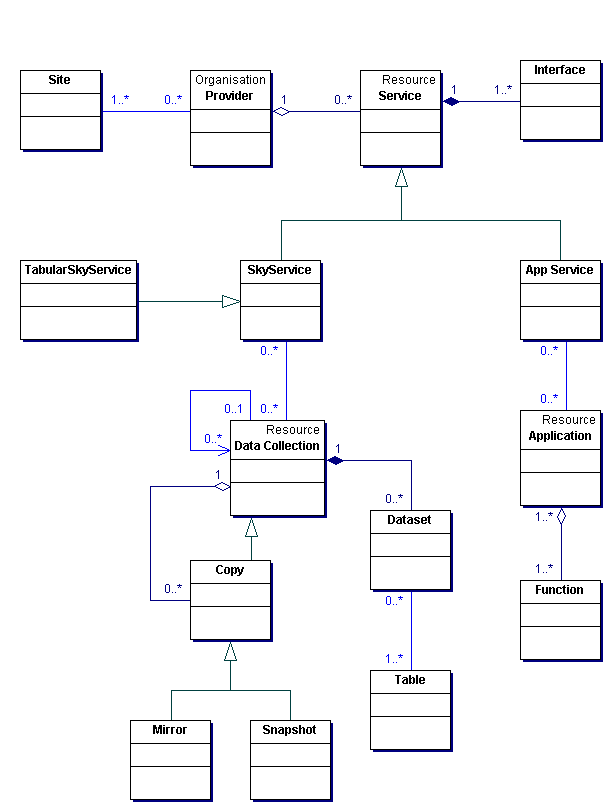
\includegraphics[height=15cm]{registry}
        \else
        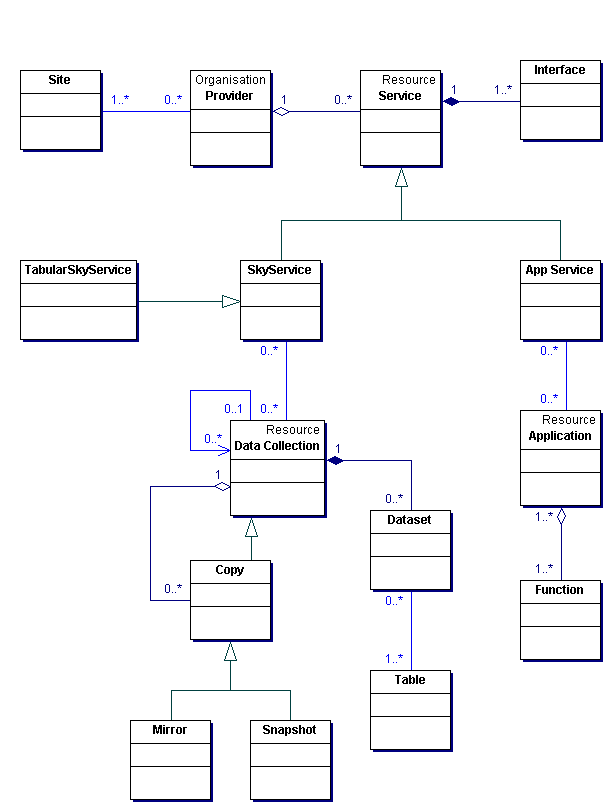
\includegraphics[bb = 92 86 545 742, height=6in]{registry}
        \fi
        \caption{UML diagram of VO-registry}
        \label{FigAir}
      \end{center}
    \end{figure}


autonomous, and its boundaries well-defined
inherently distributed

\section{Data Access Protocols}
\subsection{Cone Search Protocol}
\subsection{Simple Image Access Protocol}
\subsection{Simple Spectra Access Protocol}
\section{Data Formats}
\subsection{VOTable}
\subsection{FITS}



picture from
http://www.ivoa.net/cgi-bin/twiki/bin/view/IVOA/RegistryUseCases





%% \section{First Paragraph}
%% And now I begin my first chapter here ...

%% Here is an equation\footnote{the notation is explained in the nomenclature section :-)}:
%% \begin{eqnarray}
%% CIF: \hspace*{5mm}F_0^j(a) &=& \frac{1}{2\pi \iota} \oint_{\gamma} \frac{F_0^j(z)}{z - a} dz
%% \end{eqnarray}
%% \nomenclature[zcif]{$CIF$}{Cauchy's Integral Formula}                                % first letter Z is for Acronyms 
%% \nomenclature[aF]{$F$}{complex function}                                                   % first letter A is for Roman symbols
%% \nomenclature[gp]{$\pi$}{ $\simeq 3.14\ldots$}                                             % first letter G is for Greek Symbols
%% \nomenclature[gi]{$\iota$}{unit imaginary number $\sqrt{-1}$}                      % first letter G is for Greek Symbols
%% \nomenclature[gg]{$\gamma$}{a simply closed curve on a complex plane}  % first letter G is for Greek Symbols
%% \nomenclature[xi]{$\oint_\gamma$}{integration around a curve $\gamma$} % first letter X is for Other Symbols
%% \nomenclature[rj]{$j$}{superscript index}                                                       % first letter R is for superscripts
%% \nomenclature[s0]{$0$}{subscript index}                                                        % first letter S is for subscripts

%% \section{Second Paragraph}
%% and here I write more ...\cite{texbook}

%% \subsection{sub first paragraph}
%% ... and some more ...

%% Now I would like to cite the following: \cite{latex} and \cite{texbook}
%% and \cite{Rud73}.

%% I would also like to include a picture ...

%% \begin{figure}[!htbp]
%%   \begin{center}
%%     \leavevmode
%%     \ifpdf
%%       \includegraphics[height=6in]{aflow}
%%     \else
%%       \includegraphics[bb = 92 86 545 742, height=6in]{aflow}
%%     \fi
%%     \caption{Airfoil Picture}
%%     \label{FigAir}
%%   \end{center}
%% \end{figure}

%% % above code has been macro-fied in Classes/MacroFile.tex file
%% %\InsertFig{\IncludeGraphicsH{aflow}{6in}{92 86 545 742}}{Airfoil Picture}{FigAir}

%% So as we have now labelled it we can reference it, like so (\ref{FigAir}) and it
%% is on Page \pageref{FigAir}. And as we can see, it is a very nice picture and we
%% can talk about it all we want and when we are tired we can move on to the next
%% chapter ...

I would also like to add an extra bookmark in acroread like so ...
\ifpdf
  \pdfbookmark[2]{bookmark text is here}{And this is what I want bookmarked}
\fi
% ------------------------------------------------------------------------


%%% Local Variables: 
%%% mode: latex
%%% TeX-master: "../thesis"
%%% End: 
